\documentclass[12pt, letterpaper]{article}

\usepackage{amsmath, enumerate, comment, graphicx}
\allowdisplaybreaks[1]
%\usepackage[showframe]{geometry}
\usepackage{layout}
\DeclareMathOperator*{\argmin}{argmin}
\DeclareMathOperator*{\argmax}{argmax}
\newcommand{\bv}[1]{\mathbf{#1}}

\title{CS 676\\ Final Project Appendix}

\author{Josh Wheeler, Yotam Barnoy}

\setlength{\voffset}{-0.75in}
\setlength{\headsep}{5pt}
\setlength{\hoffset}{-0.5in}
\setlength{\textwidth}{450pt}

\begin{document}%\layout

\maketitle

This document serves as an appendix to the presentation on the final project. Refer to that document for details.

\section {Derivations of Gradient }

Likelihood of datum m:

\begin{align*}
    L = &\exp ( \sum_{t=2}^{T} \sum_{i=1}^{F}  \lambda_i f_i (y_t^m, y_{t-1}^m, x^m) ) / Z_{x^m}\\
    \text{Log Likelihood:}\\
    \text{LL} &= \sum_{t=2}^{T} \sum_{i=1}^{F}  \lambda_i f_i (y_t^m, y_{t-1}^m, x^m)   -  \log Z_{x^m}\\
    \frac{\partial \text{LL}}{\partial {\lambda_i}} &= \sum_{t=2}^{T}  f_i (y_t^m, y_{t-1}^m, x^m) - \frac{\partial z}{\partial \lambda_i} Z\\
                   &=  \sum_{t=2}^{T}  f_i (y_t^m, y_{t-1}^m, x^m) - (1 / Z) \sum_{y'} \exp ( \sum_{t=2}^{T} \sum_{i=1}^{F}  \lambda_i f_i (y'_t^m, y'_{t-1}^m, x^m) )  \sum_{t=2}^{T}  f_i (y'_t^m, y'_{t-1}^m, x^m)\\
                   &=  \sum_{t=2}^{T}  f_i (y_t^m, y_{t-1}^m, x^m) -  \sum_{y'} (1 / Z) \exp ( \sum_{t=2}^{T} \sum_{i=1}^{F}  \lambda_i f_i (y'_t^m, y'_{t-1}^m, x^m) )  \sum_{t=2}^{T}  f_i (y'_t^m, y'_{t-1}^m, x^m)\\
                   &=  \sum_{t=2}^{T}  f_i (y_t^m, y_{t-1}^m, x^m) - \sum_{y'} P(y' | x^m) \sum_{t=2}^{T}  f_i (y'_t^m, y'_{t-1}^m, x^m)\\
                   &=  \sum_{t=2}^{T}  f_i (y_t^m, y_{t-1}^m, x^m) - \sum_{y'} \sum_{t=2}^{T}  P(y' | x^m)  f_i (y'_t^m, y'_{t-1}^m, x^m)\\
                   &=  \sum_{t=2}^{T}  f_i (y_t^m, y_{t-1}^m, x^m) - \sum_{t=2}^{T} \sum_{y'}   P(y' | x^m)  f_i (y'_t^m, y'_{t-1}^m, x^m)\\
                   &=  \sum_{t=2}^{T}  f_i (y_t^m, y_{t-1}^m, x^m) - \sum_{y'}   P(y' | x^m)  f_i (y'_t^m, y'_{t-1}^m, x^m)\\
\end{align*}

Where the term on the right is expected value of $f_i$ with respect to the current model parameters.

\section {Graphs}

        \begin{figure}[ht]
            \center
            \caption{Weights of feature functions}
            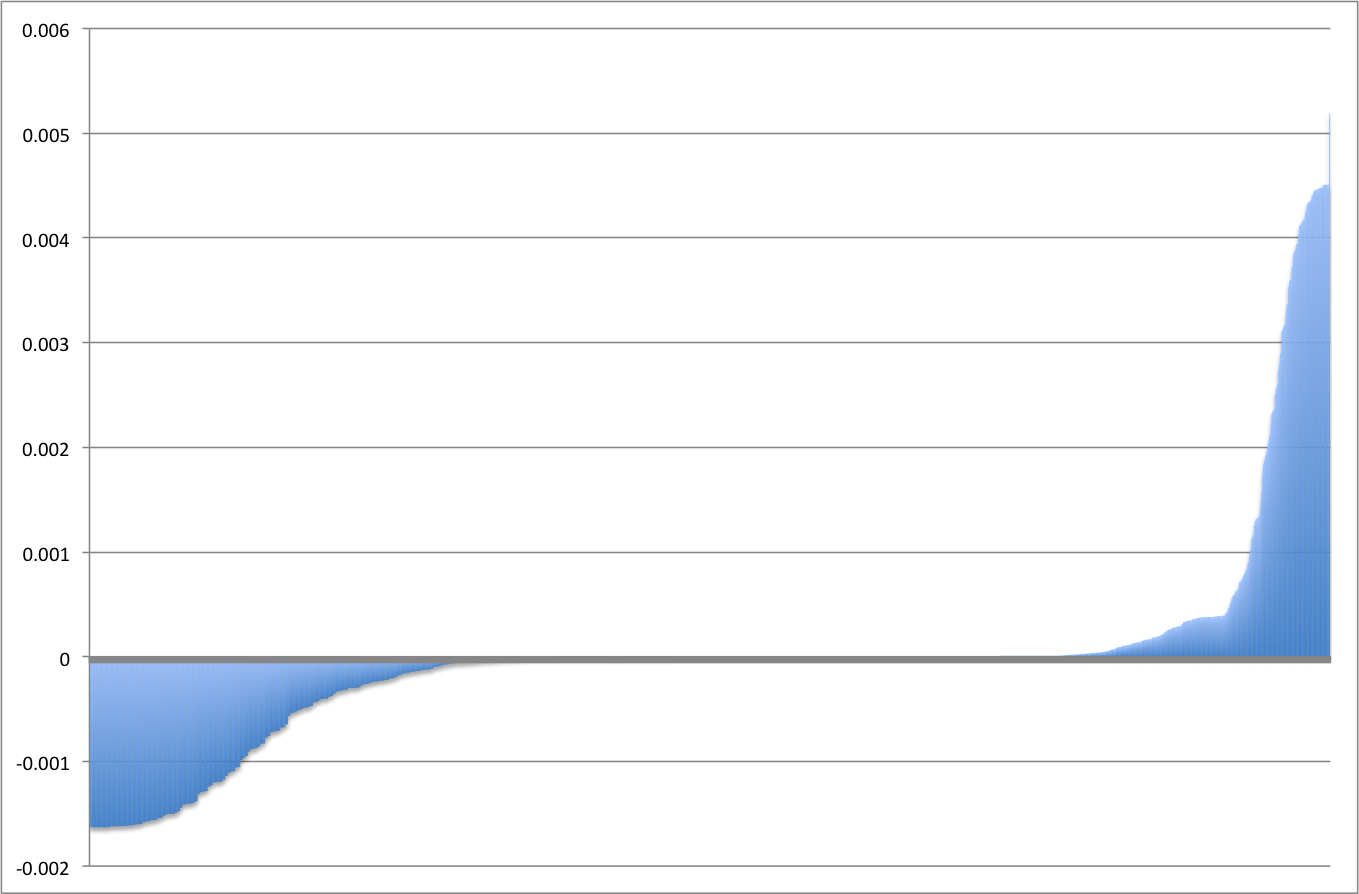
\includegraphics[scale=0.5]{ml_weights}\\
        \end{figure}

        \begin{figure}[ht]
            \center
            \caption{Likelihoods for different sigmas}
            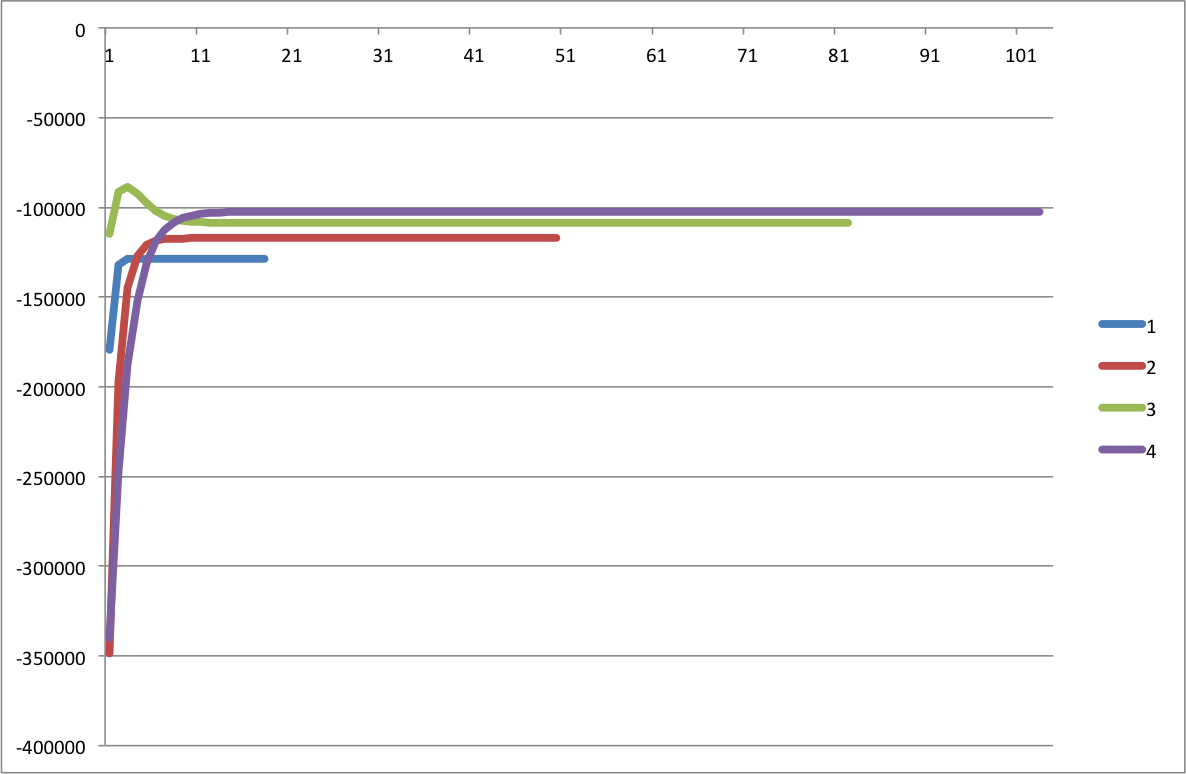
\includegraphics[scale=0.5]{ml_likelihood}\\
        \end{figure}

        These graphs demonstrate some of our results. As can be seen in the first graph, our algorithm determines that some feature functions (and therefore some features) are far more correlated with some states than are others. Additionally, the second graph demonstrates the convergence of the likelihood for different values of sigma squared (1, 2, 3 and 4 respectively) we see that convergence is slower with a higher sigma square, since the algorithm takes longer to get `trapped' at a maximum point. However, the algorithm is often able to converge to a better likelihood given more time.

\section {Sample data}
Sample data for the features chi1, chi2 and hydrogen bonds can be found in the /data directory. After building the program with `build', run `sample\textunderscore run' to see the program in action.

\section {Result data}
Please refer to the /results directory for some results we obtained using different parameters. Files called diffpart*.txt are taken from different batches of data, that is, not necessarily starting from the beginning of the data. Files called sigma*.txt vary the value of the simga square parameter, and files called window*.txt vary the window size. We also ran some batch jobs with large amounts of data, and those are still running as we speak. 

\end{document}

\begin{comment}
\end{comment}
